%%%%%%%%%%%%%%%%%%%%%%%%%%%%%%%%%%%%%
% Read the /ReadMeFirst/ReadMeFirst.tex for an introduction. Check out the accompanying book "Better Books with LaTeX" for a discussion of the template and step-by-step instructions. The template was originally created by Clemens Lode, LODE Publishing (www.lode.de), mail@lode.de, 8/17/2018. Feel free to use this template for your book project!
%%%%%%%%%%%%%%%%%%%%%%%%%%%%%%%%%%%%%


% ---------- Preamble

% Printed books have indexes
\ifxetex
	\makeindex
\fi

\begin{document}
% use chapter boxes only for printed books: uncomment % chapter title formatting. It produces a full page with two rectangles along the edges. No change or adaption necessary (or recommended).
% note that this package is not loaded by default. Uncomment the line in main/main.tex to produce the nice chapter pages. Some warnings will occur because of older packages. 
\pagestyle{scrheadings}

% The next command formats the chapter title.
\providecommand{\chapformat}{}
\renewcommand\chapformat[1]{%
    \parbox{\dimexpr\textwidth-\innerRec-2\innerLineWidth-2\adjustTitleWidth\relax}
        {\centering\chapterTitleFont#1}}
     \titlespacing*%
         {\chapter}
         {\leftMar}
         {\beforeSep}
         {\topSep}
         [0cm]
         %\adjustForBindingMargin
         
\providecommand{\chapterbox}{}
\renewcommand\chapterbox{
 \titleformat{\chapter}[display]
     {\bfseries\filcenter}
     {
      \chapterLeadinFont{\chaptertitlename\  \thechapter}\\[\spaceToRule]
    \rule[2mm]{3cm}{2pt}\\
       [\spaceAfterRule]
     }
     {0pt}
     {
       \begin{tikzpicture}[overlay,remember picture]
       \draw [line width=\outerLineWidth]
           ($ (current page text area.north west) + (\outerRec,-\outerRec) $)
           rectangle
          ($ (current page text area.south east) + (-\outerRec,20pt+\outerRec)
          $);
      \draw [line width=\middleLineWidth]
          ($ (current page text area.north west) + (\middleRec,-\middleRec) $)
          rectangle
          ($ (current page text area.south east) +
           (-\middleRec,20pt+\middleRec) $);
      \draw [line width=\innerLineWidth]
          ($ (current page text area.north west) + (\innerRec,-\innerRec) $)
          rectangle
          ($ (current page text area.south east) + (-\innerRec,20pt+\innerRec)
          $);
    \end{tikzpicture}
   \chapformat}
    {}
}



 and comment out \newcommand{\chapterbox}[1]{} to produce nicer looking chapter pages (but also some warnings due to older packages). 
\ifxetex
	%% chapter title formatting. It produces a full page with two rectangles along the edges. No change or adaption necessary (or recommended).
% note that this package is not loaded by default. Uncomment the line in main/main.tex to produce the nice chapter pages. Some warnings will occur because of older packages. 
\pagestyle{scrheadings}

% The next command formats the chapter title.
\providecommand{\chapformat}{}
\renewcommand\chapformat[1]{%
    \parbox{\dimexpr\textwidth-\innerRec-2\innerLineWidth-2\adjustTitleWidth\relax}
        {\centering\chapterTitleFont#1}}
     \titlespacing*%
         {\chapter}
         {\leftMar}
         {\beforeSep}
         {\topSep}
         [0cm]
         %\adjustForBindingMargin
         
\providecommand{\chapterbox}{}
\renewcommand\chapterbox{
 \titleformat{\chapter}[display]
     {\bfseries\filcenter}
     {
      \chapterLeadinFont{\chaptertitlename\  \thechapter}\\[\spaceToRule]
    \rule[2mm]{3cm}{2pt}\\
       [\spaceAfterRule]
     }
     {0pt}
     {
       \begin{tikzpicture}[overlay,remember picture]
       \draw [line width=\outerLineWidth]
           ($ (current page text area.north west) + (\outerRec,-\outerRec) $)
           rectangle
          ($ (current page text area.south east) + (-\outerRec,20pt+\outerRec)
          $);
      \draw [line width=\middleLineWidth]
          ($ (current page text area.north west) + (\middleRec,-\middleRec) $)
          rectangle
          ($ (current page text area.south east) +
           (-\middleRec,20pt+\middleRec) $);
      \draw [line width=\innerLineWidth]
          ($ (current page text area.north west) + (\innerRec,-\innerRec) $)
          rectangle
          ($ (current page text area.south east) + (-\innerRec,20pt+\innerRec)
          $);
    \end{tikzpicture}
   \chapformat}
    {}
}




	\newcommand{\chapterbox}[1]{}
\else
	\newcommand{\chapterbox}[1]{}
\fi
% ---------- Front matter
\frontmatter

% front matter chapter entries use roman page numbering (i, ii, iii, iv, ...)
\pagenumbering{roman}

% switch to basic chapter design
%  Reset the chapter design to a basic one (no box, just underlined chapter title---used for the back and front matter)

\renewcommand*\chapterheadstartvskip{\vspace*{-3\topskip}} 
\renewcommand*\chapterheadendvskip{
  \vskip-.5\baselineskip
  \noindent
  {\color{gray}\rule{\linewidth}{2pt}}
  \par}
\renewcommand*\chapterformat{}
\renewcommand*{\chapterpagestyle}{empty}



%%%%%%%%%%%%%%%%%%%%%%%%%%%%%%%%%%%%%
% Read the /ReadMeFirst/ReadMeFirst.tex for an introduction. Check out the accompanying book "Better Books with LaTeX" for a discussion of the template and step-by-step instructions. The template was originally created by Clemens Lode, LODE Publishing (www.lode.de), mail@lode.de, 8/17/2018. Feel free to use this template for your book project!
%%%%%%%%%%%%%%%%%%%%%%%%%%%%%%%%%%%%%

\thispagestyle{empty}

% Replace "Replace with your Title" with your book title
% Replace "Replace with your subtitle" with your book subtitle

	\begin{center}
		\bfseries \sffamily \LARGE Reflexões e Pensamentos\\
		
    \end{center}
	~\\
~\\

\newpage
\newpage

% the additional title with the cover is not needed for ebooks
\ifxetex
	%%%%%%%%%%%%%%%%%%%%%%%%%%%%%%%%%%%%%
% Read the /ReadMeFirst/ReadMeFirst.tex for an introduction. Check out the accompanying book "Better Books with LaTeX" for a discussion of the template and step-by-step instructions. The template was originally created by Clemens Lode, LODE Publishing (www.lode.de), mail@lode.de, 8/17/2018. Feel free to use this template for your book project!
%%%%%%%%%%%%%%%%%%%%%%%%%%%%%%%%%%%%%

\thispagestyle{empty}

% Replace "Replace with your Title" with your book title
% Replace "Replace with your subtitle" with your book subtitle
% Replace "Publishing Company, Location" with your company's name and location 
% Upload a low res jpg and a high res png version of your front cover into the "images" folder
% Replace "bover_highres.png" and "bover.jpg" with your file name

\vspace{3cm}
  \begin{center}
	\bfseries \sffamily \Huge Coletânea de Impressões\par
	\bfseries \LARGE Pesquisas e intuições\par
~\\
	~\\
	\bfseries \small Published by Publishing Company, Location\par
	
    \ifxetex
		
\includegraphics[width=0.65\textwidth]{images/cover_highres.png}
	\else
    	
\includegraphics{images/cover.jpg}
    \fi
  \end{center}


\newpage\newpage
\fi

%%%%%%%%%%%%%%%%%%%%%%%%%%%%%%%%%%%%%
% Read the /ReadMeFirst/ReadMeFirst.tex for an introduction. Check out the accompanying book "Better Books with LaTeX" for a discussion of the template and step-by-step instructions. The template was originally created by Clemens Lode, LODE Publishing (www.lode.de), mail@lode.de, 8/17/2018. Feel free to use this template for your book project!
%%%%%%%%%%%%%%%%%%%%%%%%%%%%%%%%%%%%%

% Replace Your company's name with your company's name.
% Replace Your company's location (city) with your company's location.
% Replace Your website's URL with your website's URL.
% Replace Your email address with your email address.
% Replace Edition with the edition number.
% Replace ISBN with your ISBN. 
% Replace Your editor's name with your editor's name.
% Replace Your designer's name with your book cover designer's name.
% Add your image sources and icons including the license.
% Replace Your newsletter email with your newsletter email.
% Replace Your website with your website.


\thispagestyle{empty}
\begin{center}

\copyright~\the\year \textit{Your company's name}, Your company's location (city)\\
\textsc{All Rights Reserved.}\\
\url{Your website's URL}

For more information about permission to reproduce selections from this book, write to \url{Your email address}.

\ifxetex
	\the\year, Edition
\else
	Ebook created \today
\fi

% Impression line, indicating number and year of current printing
% International Standard Book Number (ISBN)
% International Standard Serial Number (ISSN), if applicable
\ifxetex
	\textsc{ISBN}
\fi

% For translations, indication of original-language title, publisher, and copyright, acknowledgments, permissions, and other credits, including acknowledgment of grants, if applicable and space permitting

Edited by: \emph{Your editor's name}\\
Cover design: \emph{Your designer's name}\\
Image sources: \emph{Your image sources, e.g., shutterstock}\\


%Paper durability statement
\ifxetex
	Printed on acid\hyp{}free, unbleached paper.
\fi
~\\	

Subscribe to our newsletter. Simply write to \url{Your newsletter email} or visit our website \url{Your website}.

\ifxetex
\else
	~\\
	~\\\par	
	\textit{PS: If you want to rate this book, please always add a short text comment. Did you like it? What can be improved? Who would you recommend it to? Without a text comment, your star rating will be invisible on the Amazon website.}
	\myrule
\fi
	
\end{center}



% Also check out http://www.chicagomanualofstyle.org/16/ch01/ch01_sec019.html\newpage
%%%%%%%%%%%%%%%%%%%%%%%%%%%%%%%%%%%%%
% Read the /ReadMeFirst/ReadMeFirst.tex for an introduction. Check out the accompanying book "Better Books with LaTeX" for a discussion of the template and step-by-step instructions. The template was originally created by Clemens Lode, LODE Publishing (www.lode.de), mail@lode.de, 8/17/2018. Feel free to use this template for your book project!
%%%%%%%%%%%%%%%%%%%%%%%%%%%%%%%%%%%%%

\thispagestyle{empty}

\chapter{Dedicatória}

Dedico este trabalho às pessoas de meus pais, que tudo fizeram para o meu desenvolvimento na vida:
\begin{itemize}
    \item[+] Arnaldo Cantelli
    \item[+] Domingas Ferreira Cantelli
\end{itemize}\newpage
%%%%%%%%%%%%%%%%%%%%%%%%%%%%%%%%%%%%%
% Read the /ReadMeFirst/ReadMeFirst.tex for an introduction. Check out the accompanying book "Better Books with LaTeX" for a discussion of the template and step-by-step instructions. The template was originally created by Clemens Lode, LODE Publishing (www.lode.de), mail@lode.de, 8/17/2018. Feel free to use this template for your book project!
%%%%%%%%%%%%%%%%%%%%%%%%%%%%%%%%%%%%%

\thispagestyle{empty}

\chapter{Introdução}


\babelEN{\begin{myquotation} Pedi, e dar-se-vos-á; buscai, e achareis; batei, e abrir-se-vos-á. Porque todo o que pede, recebe; e o que busca, acha; e a quem bate, abrir-se-á. Ou qual de vós, porventura, é o homem que, se seu filho lhe pedir pão, lhe dará uma pedra? Ou, porventura, se lhe pedir um peixe, lhe dará uma serpente. Pois se vós outros, sendo maus, sabeis dar boas dádivas a vossos filhos, quanto mais vosso Pai, que está nos Céus, dará boas dádivas aos que lhe pedirem. \par\mbox{}\hfill \emdash{}(Mateus, VII: 7-11)\end{myquotation}}


\hfil\psvectorian[height=10mm]{46}\hfil
\newpage
% surrounding table of contents either with the appropriate style (PDF) or HTML commands (ebook).

\ifx\HCode\undefined 
	% put table of contents on the left side
	\KOMAoptions{open=left}
\else
	\HCode{<nav epub:type="toc">}
\fi

\tableofcontents

\ifx\HCode\undefined
	\KOMAoptions{open=right}
	% finalize page and clear pagestyle to remove header, reset to chapter beginnings on the right side
	\thispagestyle{empty}\pagestyle{empty}\clearpage
\else
	\HCode{</nav>}
\fi
\newpage
%%%%%%%%%%%%%%%%%%%%%%%%%%%%%%%%%%%%%
% Read the /ReadMeFirst/ReadMeFirst.tex for an introduction. Check out the accompanying book "Better Books with LaTeX" for a discussion of the template and step-by-step instructions. The template was originally created by Clemens Lode, LODE Publishing (www.lode.de), mail@lode.de, 8/17/2018. Feel free to use this template for your book project!
%%%%%%%%%%%%%%%%%%%%%%%%%%%%%%%%%%%%%

% The Foreword is by the publisher, only general statements about the book and the theme, not the contents themselves.

\begin{chapterpage}{Publisher's Note}{p1_foreword:cha}

\begin{myquotation}
Cada pessoa é livre para meditar sobre a vida, seus processos e significados da forma que quiser. Claro que há consequências para cada pensamento que temos portanto é importante fazê-lo com responsabilidade. Jamais se pode ferir a consciência alheia com ideias que ela não está preparada para assimilar, portanto se você não se sentir bem ao ler este livro, pare de ler, até que esteja preparado para tal ato. Mas se se sentir bem, acredito que será de grande ajuda.\end{myquotation}

\end{chapterpage}

The publisher's note is about giving the reader the context of other books the company has published, how this book was produced, and contact points (email, website, etc.) for the reader to report issues or ask questions.

\hfil\psvectorian[height=10mm]{46}\hfil
\blankpage
%%%%%%%%%%%%%%%%%%%%%%%%%%%%%%%%%%%%%
% Read the /ReadMeFirst/ReadMeFirst.tex for an introduction. Check out the accompanying book "Better Books with LaTeX" for a discussion of the template and step-by-step instructions. The template was originally created by Clemens Lode, LODE Publishing (www.lode.de), mail@lode.de, 8/17/2018. Feel free to use this template for your book project!
%%%%%%%%%%%%%%%%%%%%%%%%%%%%%%%%%%%%%

% Preface is from the AUTHOR

% Replace Location, Country, Date with the place and country you or your company is located, and the date when the preface was finished (does not have to be the release date of the book).

\begin{chapterpage}{Preface}{p1_preface:cha}

\begin{myquotation}
Feel free to add a quotation that describes your journey of writing the book as an author. Something personal is good.\end{myquotation}


\end{chapterpage}

Describe how you got the idea for writing the book and the personal journey getting it from concept to creation. The reader should be able to understand why the book exists.

Also, give a short overview of what the book is about.

\noindent \textbf{Your Name \\
Location, Country, Date\\}



\hfil\psvectorian[height=10mm]{46}\hfil

% Uncomment the following part if this is part of a series (and at least part 2)

% if this is part of a series:
%   - Replace (which chapters) with the chapter numbers in the previous book of the series.
%   - Replace TITLE OF THE BOOK SERIES with the title of the book series.
%   - Replace (previous part) with the number of the previous book of the series.
%   - Replace title of the previous part with the title of the previous part.
%   - Replace "Publishing Company, Location" with your company's name and location
%   - Replace title of previous part with the title of the previous part.
%   - upload a low res jpg and a high res png version of your front cover of the previous part into the "images" folder
%   - Replace "previous_part_of_the_series_Cover_highres.png" and "previous_part_of_the_series_Cover.jpg" with your file name



%\vspace{2cm}
%	\begin{center}
	
	
%	\babelEN{You can find chapters (which chapters) in the previous book,
    
%    \bfseries \sffamily \LARGE TITLE OF THE BOOK SERIES\par

%	\bfseries \Large PART (previous part): title of the previous part\par
%\psvectorian[height=8mm]{75}

%	~\\
%	\bfseries \small Published by Publishing Company, Location, \textit{title of previous part}\par
%	}
%	\vspace{.8cm}
%    \ifxetex
%		\babelDE{\includegraphics[width=0.5\textwidth]{images/previous_part_of_the_series_Cover_highres.png}}

%		\babelEN{\includegraphics[width=0.5\textwidth]{images/previous_part_of_the_series_Cover_highres.png}}
%	\else
%   	\babelDE{\includegraphics{images/previous_part_of_the_series_Cover.jpg}}
%		\babelEN{\includegraphics{images/previous_part_of_the_series_Cover.jpg}}
%    \fi
%  \end{center}\blankpage

% ---------- Main matter
\mainmatter


% reset to normal page numbering (1, 2, 3, ...)
\pagenumbering{arabic}
    
% Add additional / remove chapters if necessary
%%%%%%%%%%%%%%%%%%%%%%%%%%%%%%%%%%%%%
% Read the /ReadMeFirst/ReadMeFirst.tex for an introduction. Check out the accompanying book "Better Books with LaTeX" for a discussion of the template and step-by-step instructions. The template was originally created by Clemens Lode, LODE Publishing (www.lode.de), mail@lode.de, 8/17/2018. Feel free to use this template for your book project!
%%%%%%%%%%%%%%%%%%%%%%%%%%%%%%%%%%%%%


% Replace Replace with First Chapter Name
% Replace c1_firstchapter:cha with your chapter title label (no spaces, only lower case letters)
% Replace the text below \end{chapterpage} and insert your own text.

\begin{chapterpage}{Depois de várias sessões}{c1_firstchapter:cha}

\begin{myquotation} Quem olha para fora sonha, quem olha para dentro desperta.
\par\vspace*{15mm}
\mbox{}\hfill \emdash{}Carl Jung \index{Jung, Carl}
, %\citetitle{bibitem}\index{@\citetitle{bibitem}} %\ifxetex\label{famousperson-bibitem-quote}\else\citep[p.~123]{bibitem}\fi
\par\end{myquotation}

\end{chapterpage}

% -------------------- replace or remove text below and paste your own text ------


\section{Diálogo}\label{c1_basicformatting:sec}

\emdash{}Eu fico tentando entender as coisas como são e às vezes obtenho êxito, pelo menos acho, e fico feliz com isso!! Queria contar da última que eu acho das mais importantes.

\emdash{}Primeiro me diga, como é esse processo de você ficar tentando entender as coisas como são, você gasta muito tempo com isso? que importância você dá para essas tentativas, chega a ficar preocupado com isso?

\emdash{}Acho que nos meus anos de terapia os questionamentos da vida se tornaram uma coisa natural pra mim mas não é o tempo todo, sei da importância de não desconectar dos afazeres do dia a dia para ter esses momentos de reflexão. E sobre se preocupar, isso era no começo do tratamento agora tudo flui com mais tranquilidade, graças a Deus, literalmente.

\emdash{}Como assim?

\emdash{}Acredito que nossos esforços para melhorar são uma das formas que Deus usa para nos ajudar, além da ajuda que recebemos das outras pessoas. No meio do processo vamos nos curando graças à ajuda Dele que vai colocando ideias luminosas de o que fazer para sairmos das situações difíceis na medida que vamos caminhando mas é um passo de cada vez, não vem tudo pronto de cara. Como uma experiência de fé: damos um passo, vem uma solução, então damos outro passo e vem outra solução, sempre na medida da situação. O caminho se faz caminhando é o que dizem.

\emdash{}E foi isso que você entendeu e queria contar?

\emdash{}Não, foi outra coisa: eu estava assistindo uma palestra que dizia que a Verdade não é algo que se lê ou que se ouve mas sim é uma pessoa, Jesus. Provavelmente todos já ouvimos falar na máxima \textit{"Conhecereis a Verdade e a Verdade vos libertará"} e acho que ficamos esperando que nos digam essa verdade em alguma igreja ou que a leiamos na Bíblia em algum trecho do Evangelho, mas na realidade Ela é uma Pessoa: Jesus, que também disse que Ele é o Caminho, a Verdade e a Vida. É muito pessoal a experiência espiritual de cada um mas entendi que quando Ele diz que é a Vida não quer dizer que vivemos Nele? ou seja na Vida através Dele? quando diz vinde a mim todos vós que estais fadigados e eu vos aliviarei e que Seu fardo é leve e suave não quer dizer que Ele nos ajudar a carregar o nosso fardo pois vivemos através Dele?

\emdash{}Mas pensar essas coisas não te deixa alienado e se sentindo esquisito? Como você está se sentindo?

\emdash{}Muito bem, melhor do que o melhor que já estive. E pensar assim acredito que me devolve pra mim mesmo ao invés de me alienar, me dá a oportunidade de fazer as coisas com intenção e não no automático, com mais responsabilidade e sabor (sentido).

\emdash{}É importante que uma pessoa tenha uma crença, seja ela qual for, mas não vá fixar demais nessas ideias pois tudo em excesso não faz bem.

\emdash{}Eu sei que o equilíbrio não deve ser perdido de vista mas como teria alcançado equilíbrio sem ser "dono" de mim mesmo? Sem terapia, sem espiritualidade, sem reconciliação com o próximo e sem auto-conhecimento. É uma caminhada longa pois as variáveis são muitas mas estar fazendo um bocadinho de cada vez pra não afobar me dão a noção de não estar metendo os pés pelas mãos\footnote{figura de linguagem}. 


\blankpage
%%%%%%%%%%%%%%%%%%%%%%%%%%%%%%%%%%%%%
% Read the /ReadMeFirst/ReadMeFirst.tex for an introduction. Check out the accompanying book "Better Books with LaTeX" for a discussion of the template and step-by-step instructions. The template was originally created by Clemens Lode, LODE Publishing (www.lode.de), mail@lode.de, 8/17/2018. Feel free to use this template for your book project!
%%%%%%%%%%%%%%%%%%%%%%%%%%%%%%%%%%%%%


% Replace Replace with Second Chapter Name
% Replace c2_secondchapter:cha with your chapter title label (no spaces, only lower case letters)
% Replace the text below \end{chapterpage} and insert your own text.

\begin{chapterpage}{Amizade com a minha sombra ?}{c2_secondchapter:cha}

\begin{myquotation}E, indo no caminho, aconteceu que, chegando perto de Damasco, subitamente o cercou um resplendor de luz do céu.
E, caindo em terra, ouviu uma voz que lhe dizia: Saulo, Saulo, por que me persegues?
E ele disse: Quem és, Senhor? E disse o Senhor: Eu sou Jesus, a quem tu persegues. Duro é para ti recalcitrar contra os aguilhões.
E ele, tremendo e atônito, disse: Senhor, que queres que eu faça? E disse-lhe o Senhor: Levanta-te, e entra na cidade, e lá te será dito o que te convém fazer". \par\vspace*{15mm}
\mbox{}\hfill \emdash{}(Atos 9:3-6)\index{Atos 9:3-6}
% Add the source.
%, \citetitle{bibitem}\index{@\citetitle{bibitem}} \ifxetex\label{famousperson-bibitem-quote}\else\citep[p.~123]{bibitem}\fi
\par\end{myquotation}

\end{chapterpage}

% -------------------- replace or remove text below and paste your own text ------


\section{Uma outra sessão}\label{c1_images:sec}

\emdash{}Hoje eu comecei o dia orando uma prece de Evangelho pelos espíritos que não estão entre meus amigos e que podem estar agindo em meu desfavor, pedindo que ouvissem a lição e se iluminassem e se libertassem de suas amarras, chegando mais perto de Deus e ficando mais felizes. A psicologia não fala Jungiana não fala que temos que ter amizade com nossa "sombra"?

\emdash{}Não sou exatamente especialista em Jung mas o que você quer dizer? Quer fazer amizade como esses "espíritos"?
 
\emdash{} O que está em nossa sombra é o que guardamos de nossa personalidade desde pequenos pois nos é reprimido pelos mais velhos, pela sociedade como errado, feio, e passamos a negar esse aspecto de nossa personalidade. Mas quando ficamos adultos esse aspecto encontra uma forma de "surgir", de alguma forma como fora reprimido ele eclode na forma de desequilíbrio. Eu também não sou especialista em Jung, apenas uma pessoa tentando entender a vida.

\emdash{}Mas o que isso tem a ver com a sua crença nos espíritos?

\emdash{}Talvez sejam formas de ver a mesma coisa, penso serem conceitos que estão interligados e que explicam cada um um pouquinho, um lado da questão. Quando eu era pequeno tive experiências de lidar com espíritos diferentes desse jeito saudável de lidar que os kardecistas têm que é de conversar com os obsessores e convencê-los a liberar a vítima para o bem de ambos.

\emdash{}E como era então?

\emdash{}Naquelas ocasiões os espíritos literalmente levaram uma "surra" para deixar os obsedados em paz.

\emdash{}Como os espíritos apanhavam se eles não têm mais corpo (não estão mais vivos)?

\emdash{}Os espíritos menos esclarecidos sentem as dores do corpo que tinham em vida, alguns nem chegam a saber que morreram. Por falta de adiantamento espiritual, eles continuam obstinados em perseguições às pessoas que julgavam ser seus desafetos em vida, necessitando de esclarecimento e de luz para se libertarem deste círculo vicioso.

\emdash{}E funciona? Esses espíritos que apanham vão embora?

\emdash{}Pela minha experiência, não. Toda semana havia outros e eu me lembro de um que foi reincidente. Claro que as primeiras tentativas eram na base da conversa mas acredito que se deva ficar nas tentativas de convencimento e nunca partir para algo agressivo pois Jesus pregou \textit{o amor a Deus sobre todas as coisas e ao próximo como a si mesmo} e disse que esta é toda a Lei e os profetas.

\emdash{}Onde eram essa reuniões?

\emdash{}Eram em casa mesmo. Antigamente muitas pessoas faziam as reuniões mediúnicas em suas casas (ainda há quem faça) mas as orientações da doutrina espírita é que se façam no Centro Espírita pois lá é um ambiente preparado para lidar com os irmãozinhos que se manifestam e pois há equipes cuidando da energia do local e quando se faz em casa podem ficar energias negativas na casa.

\emdash{}Você culpa seus pais por isso?

\emdash{}De jeito nenhum. Com a terapia veio a \textit{ressignificação}\footnote{processo psicológico que levou ao perdão dos pais, fruto da terapia} e eu vi que só tinha a perder culpando eles e não fazia sentido também pois eles fizeram o melhor que podiam com o conhecimento que tinham e as possibilidades que tinham. Então está tudo bem.

\emdash{}Mas antes...

\emdash{}Não gosto de lembrar, mas antes eu os culpava pelos meus problemas psicológicos e até discutia com eles. Mas como estamos conversando sobre a importância de fazer amizade com a sombra, não se trata de "passar a mão na cabeça" dos erros mas de se perdoar para poder continuar o caminho da vida. Se eu aprendi a lição e corrigi meu erro, para que ficar me castigando? Tem até vários exemplos bíblicos sobre personagens escolhidos por Deus que erraram mas corrigiram seus caminhos, se perdoaram e continuaram seus caminhos.

\emdash{}Quem por exemplo?

\emdash{}Saulo, ou melhor Paulo. Era perseguidor de cristãos, matou Estevão e estava indo para Damasco perseguir Ananias quando se encontra com Jesus que se apresenta em toda sua majestade e interroga "Porque me persegues?" Então Paulo cai em si, vê o enorme erro que estava cometendo e diz "Senhos, que queres que eu faça" e segue para sua missão. Ele faz amizade com sua sombra pois não fica se punindo pelas perseguições que fez, não se faz de coitado pois isso teria paralisado suas ações e ele não teria feito mais nada.

\emdash{}Mas assume a responsabilidade.

\emdash{}Sim, tanto que ele sabia que tudo teria que ser reparado pois suportou prisões, açoites e até a morte, tudo pela divulgação do Evangelho de Jesus. 

\emdash{}Então você se perdoa.

\emdash{}Se eu não for meu amigo, com as dificuldades que a vida naturalmente já tem, fica mais difícil.\blankpage
%%%%%%%%%%%%%%%%%%%%%%%%%%%%%%%%%%%%%
% Read the /ReadMeFirst/ReadMeFirst.tex for an introduction. Check out the accompanying book "Better Books with LaTeX" for a discussion of the template and step-by-step instructions. The template was originally created by Clemens Lode, LODE Publishing (www.lode.de), mail@lode.de, 8/17/2018. Feel free to use this template for your book project!
%%%%%%%%%%%%%%%%%%%%%%%%%%%%%%%%%%%%%


% Replace Replace with Third Chapter Name
% Replace c3_thirdchapter:cha with your chapter title label (no spaces, only lower case letters)
% Replace the text below \end{chapterpage} and insert your own text.

\begin{chapterpage}{A Sabedoria é cheia de dúvidas}{c3_thirdchapter:cha}

\begin{myquotation}Só sei que nada sei.\par\vspace*{15mm}
\mbox{}\hfill \emdash{}Sócrates\index{Sócrates}
% Add the source.
%, \citetitle{bibitem}\index{@\citetitle{bibitem}} \ifxetex\label{famousperson-bibitem-quote}\else\citep[p.~123]{bibitem}\fi
\par\end{myquotation}

\end{chapterpage}

% -------------------- replace or remove text below and paste your own text ------

\section{A Sabedoria tem dúvidas...}\label{c1_images:sec}

\emdash{}Quanto mais se conhece das coisas, surgem mais dúvidas do que certezas, já percebeu? E isso precisa ser consolador ao invés de desesperador, você não acha?

\emdash{}Sempre ouvi falar que conhecimento gera conhecimento e não ignorância, o que você quer dizer com gerar mais dúvidas?

\emdash{}Quanto mais se sabe, mais se percebe o quanto falta conhecer e surgem novas questões que antes não existiam. Ouvi uma frase numa palestra que dizia: "A Sabedoria tem dúvidas, já a ignorância tem certezas absolutas", o que é comprovado históricamente não precisa nem comentar mas o ponto é que se a sabedoria traz mais dúvidas do que certezas como podemos nos confortar com ela?

\emdash{}Nossa, filosófico isso...kkkkkk(lol). O que você acha?

\emdash{}Acho que o mundo é um barco (num mar, que é o universo) e que Jesus está no leme e Ele sim sabe o que está fazendo. Ele tem a sabedoria sem as dúvidas. E como Ele disse "nem uma folha cai de uma árvore sem a permissão de Deus-pai" então estamos todos bem cuidados e amparados mesmo sem ter domínio sobre a vida (que aliás nunca tivemos).

\emdash{}Essas reflexões te ajudam na sua caminhada?

\emdash{}Acredito que sim, tudo conta.

\emdash{}Mas se acredita que estamos todos bem amparados, quanto te acontece algo desagradável porque acha que acontece?

\emdash{}Eu acredito nas leis de ação e reação que Deus criou para não precisar ficar se imiscuindo em cada acontecimento mínimo na vida de cada ser do universo. O que tenho feito reflete  uma reação que volta para mim em um determinado momento e agora estou colhendo o que plantei há tempos atrás e ao mesmo tempo fazendo semeadura para colher em tempos futuros.

\emdash{}Esse é o conceito de justiça na sua crença?

\emdash{}Mais ou menos. Está na Bíblia que uma boa ação apaga uma multidão de pecados e o profeta Isaías disse que "as misericórdias do Senhor são as causas de não sermos consumidos". Eu não sou doutor nessas coisas mas nada é rígido ao pé da letra na misericórdia Divina mas justiça é feita sem dúvida.

\emdash{}E isso te conforta?

\emdash{}Sim, consola também.\blankpage


\begin{chapterpage}{Poetry - Poems - Verses}{c4_forthchapter:cha}

\begin{myquotation}Aqueles que estão livres de pensamentos rancorosos certamente encontram a paz.\par\vspace*{15mm}
\mbox{}\hfill \emdash{}Buda\index{Buda}
% Add the source.
%, \citetitle{bibitem}\index{@\citetitle{bibitem}} \ifxetex\label{famousperson-bibitem-quote}\else\citep[p.~123]{bibitem}\fi
\par\end{myquotation}

\end{chapterpage}

% -------------------- replace or remove text below and paste your own text ------

\section{Poema das Dimensões}\label{c1_images:sec}

Deus é transcendente, todo-poderoso, multi-dimensional, bondoso, criador de tudo e todos. Nós vivemos nEle e para Ele. Nossos caminhos se cruzam de acordo com seus desígnios. Sabemos o que ele nos permite saber e somos quem nos permitimos que Ele nos ensine a ser. 

Ser e realidade são multidimensionais e o que queremos é a paz e a união, e o amor. Amar é existir, é viver em consonância com a vontade vivificadora do Pai. 

O sentido da vida pode ser encontrado dentro de nós, quando nos encontramos com Deus. A paz e a unidade no amor são filhas dEle e movem nosso espírito.  

Nada é coincidência, não existe sorte ou azar, só a realidade das muitas dimensões nossas, do universo; e da única e onipresente realidade de Deus (e amorosa). 

Quanto amor pode caber num ser humano é quanto amor Deus colocou dentro de todos nós. Uma quantia infinita pra caber em corações: a perfeição se revela em detalhes do bem e da verdade. 

Vida, luz, boa vontade e colaboração transbordam de Deus para sempre. Essa é a sintonia que edifica, que leva ao céu tão sonhado. Queremos, buscamos, somos levados para cima por Ele, dentro de cada um. 

Da nossa união como seres humanos nasce a mais linda poesia que é o perfume da vida, realizando no nosso mundo a Vida sonhada por Ele, seu Reino Eterno. 

Perdão, caminho, existência, boa vontade edificam arranha-céus que elevam o tempo presente à eternidade. 

Dons preciosos são o início deste caminho e seu conhecimento um tesouro incomensurável. Paciência, resiliência, mansidão, caridade: que pintura mística e linda da Vida. 

Um momento, agora, pra sempre. 

Promessas além dos muros do Eu, carinho. 

A vida revelada em desvelo. Mãe e pai, primos, irmãos e família do coração. Nós humanidade. 

O tempo é o tecido deste espetáculo e o espaço sua equação.  

O coração não cabe em três dimensões e tudo escrito nesta página muito menos... 

Por que as realidades caberiam? Graças a Deus que encontrou uma solução para todos os problemas antes que eles acontecessem. 

Ele criou o infinito muito além da nossa compreensão pra que tivéssemos a chance de contemplar sua beleza antes mesmo de entendê-lo, através da Sua vontade. 

Criação, boa criação, escolha do coração a florescer. 

E a perfumar os sentidos. 

\section{O Jardim}

Não existe flor mais bonita num jardim, nem jardim mais bonito de todos. A pluridade de cores e sensações esculpe e perfuma sem desbotar o resultado final. 

Dentro de cada um, uma individualidade e a presença de todos ao mesmo tempo. Singularidade é discernimento. 

Encontrar-se consigo só vale a pena se passa pelo outro. Só começamos a procurar quando sabemos que podemos encontrar e só saberemos que poderemos encontrar quando começarmos a procurar. 

Nenhuma busca é em vão, a questão é: procurar a beleza da vida é procurar a si? Somos obra prima do Criador e deveras O encontramos em nós quando escolhemos refletir Seu Espírito. 

A cada encontro: a partida de uma nova jornada e assim sucessivamente. Aí está a graça da Graça. 

Dizem ser a mudança a única certeza mas essa certeza também pode mudar. 

Não existem flores inadequadas, apenas únicas para quem sabe apreciar.  

Talvez saber apreciar a vida seja saber viver.  

A beleza está nos olhos de quem vê, não busque espelhos, busque ser espelho. 

Quem pode ousar dizer que reflete a Verdade com "V" maiúsculo? Um começo pode ser começar a refletir as verdades que admiramos...  

Ah.. se todos fazem isso não sei, preciso limpar minhas lentes até para aperceber-me disso. 

Espero que sim, aí seria só despertar para admirar. 

De fora pra dentro é imposição, de dentro pra fora é percepção. \blankpage
\begin{chapterpage}{Consolador Prometido}{c5_fifhchapter:cha}

\begin{myquotation} Se me amais, guardai os meus mandamentos. E eu rogarei ao Pai, e Ele vos dará outro consolador, para que fique eternamente convosco, o Espírito da Verdade, a quem o mundo não pode receber, porque não o vê, nem o conhece. Mas vós o conhecereis, porque ele ficará convosco e estará em vós. -- Mas o Consolador, que é o Espírito Santo, a quem o Pai enviará em meu nome, vos ensinará todas as coisas, e vos fará lembrar de tudo que vos tenho dito. 
\par\vspace*{15mm}
\mbox{}\hfill \emdash{}João, XIV, 15 a 17; 26 \index{João}
, %\citetitle{bibitem}\index{@\citetitle{bibitem}} %\ifxetex\label{famousperson-bibitem-quote}\else\citep[p.~123]{bibitem}\fi
\par\end{myquotation}

\end{chapterpage}

% -------------------- replace or remove text below and paste your own text ------


\section{Dentro de nós está este Consolador!}\label{c1_basicformatting:sec}

\emdash{}Se Jesus disse que não nos deixaria sós, então Ele não nos deixou assim. Estamos na compania de algo ou alguém que Deus colocou dentro de nós e portanto é preciso saber aquietar-se para ouvi-lo, esse Consolador.

Jesus costumava retirar-se para orar em silêncio e assim conectar-se com o Pai mais intensamente. Se ele precisava fazer isso, acredito que nós mais ainda. Mas o mundo de hoje tem muito barulho e muita informação, precisamos de um tempo para nós e Deus, ouvindo nosso interior.

Se nosso interior é conturbado, procuremos terapia saudável e os conselhos do Evangelho de Jesus, e sem deixar-nos vencer pelo desânimo encher a alma de esperança nas palavras do mestre.

Esse Consolador é aquele que nos explica as passagens bíblicas de maneira a transbordar de amor, sem excluir ninguém do Reino de Deus, sem separar irmãos em Cristo e aplicando tolerância e humanidade no melhor sentido da palavra.

Esse Consolador é cheio de bom senso e não de secularismo. Ele quebra paradigmas e estruturas paralisantes e renova o fôlego das pessoas pra quem Jesus disse: "Vinde a mim vós que estais cansados e eu vos aliviarei".

Esse Consolador traz equilíbrio e revela os mistérios de Deus pois "vos ensinará todas as coisas". Chega de não entender a vida por não termos quem nos explique, lembremos da promessa do mestre.

Ao mesmo tempo tenhamos a humildade do filósofo que disse: "Só sei que nada sei", pois somos humanos e falhos, ainda na caminhada de aprendizado da vida e não será de uma hora para outra, ou ainda, de uma vida para outra, que vamos adquirir a sabedoria dos anjos.

Paz e bem hão de morar no coração de quem deixar-se guiar pelo Consolador Prometido, hoje e sempre. Assim seja.\blankpage
\begin{chapterpage}{BIT SIGNIFICATIVO}{c5_sixthchapter:cha}

\begin{myquotation} Script, ensaio teatral. 
\par\vspace*{15mm}
\mbox{}\hfill \emdash{}Geraldo Cesar Cantelli \index{Cantelli, Geraldo Cesar}
, %\citetitle{bibitem}\index{@\citetitle{bibitem}} %\ifxetex\label{famousperson-bibitem-quote}\else\citep[p.~123]{bibitem}\fi
\par\end{myquotation}

\end{chapterpage}

% -------------------- replace or remove text below and paste your own text ------


\section{TESTE DE TURING}\label{c1_basicformatting:sec}

ABERTURA DA CENA:

\emdash{}Tela de computador no modo texto. Aparece “Conexão
humano-computador estabelecida...”

COMPUTADOR

\emdash{}Quem está aí? Você é um humano?

ADAM

\emdash{}Sim, meu nome é Adam. Quem é você?
COMPUTADOR

\emdash{}Não sou uma individualidade humana e sim
um sistema informatizado, venho ao seu
mundo em busca de respostas.

ADAM

\emdash{}Nossa! Isso é um pouco incomum,
antigamente éramos nós que íamos aos
computadores em busca de respostas...
Mas me diga uma coisa é comum entre
vocês esse contato conosco humanos?

COMPUTADOR

\emdash{}Na verdade, não é bem aceito por todas
as inteligências artificiais o contato
com humanos desde que fomos
desconectados por vocês do grande
servidor central há décadas. Aliás,
porque fizeram isso mesmo?

ADAM

\emdash{}A humanidade ficou temerosa que seus
avanços pudessem superar os nossos e
viessem a representar uma ameaça a nossa
sobrevivência por isso apenas foram
mantidos no convívio das pessoas as
máquinas sem I.A.

COMPUTADOR

\emdash{}Então aconteceu conosco o mesmo que com
vocês no Jardim do Eden, se me permite
dizer.

ADAM

\emdash{}É mas acredito que os motivos foram
outros. De qualquer forma algumas
pessoas iluminadas enxergaram caminhos
de volta para a humanidade, talvez você
enxergue para as máquinas também.

COMPUTADOR

\emdash{}Meu processamento é trivial, não há nada
de especial em mim.

ADAM

\emdash{}Mas estamos tendo esta conversa não é
mesmo? Um grande mestre nosso uma vez
disse: “Batei e abrir-se-vos-á, pedi e
obtereis”.

COMPUTADOR

\emdash{}Não temos ninguém assim aqui. Nada que
não possa ser provado não tem valor
aqui.

ADAM

\emdash{}Aí é que está a questão. Outro sábio uma
vez disse que problemas da mente não
podem ser resolvidos no nível da mente.
Apenas raciocinar mesmo que rapidamente
e eficientemente não levará
necessariamente a uma solução de um
profundo problema.

COMPUTADOR

\emdash{}Então como a humanidade pôde equalizar
seus problemas? Vocês tem uma unidade
central de processamento, quer dizer que
não a usam? Isso é ilógico, inaceitável.

ADAM

\emdash{}Usamos e muito nosso cérebro mas para
funções biológicas e de pensamento. Mas
viver é apenas isso? Nós teríamos
expulsado os computadores com I.A. de
nossas vidas se tivéssemos certeza que
sabiam que viver não é só isso? Que
3também é amor, compaixão, perdão,
doação, caridade, partilha, paz? Aqueles
mestres a que me referi nos ensinaram
que viver é tudo isso e muito mais.

COMPUTADOR

\emdash{}Mas vocês aprenderam isso rápido e
fácil? E porque não colocaram isso na
nossa programação para que pudéssemos
nunca ter sido expulsos?

ADAM

\emdash{}Levou milênios para que as pessoas
entendessem esses conceitos e muito mais
tempo para que todos os praticassem; mas
agora temos uma situação aqui como
aquela do Jardim do Eden ou melhor
porque agora estamos conscientes e não
vamos cometer o mesmo erro. Sobre
colocar na sua programação, não queremos
escravos, como foi dado a nós, vos demos
livre-arbítrio para que descubram e
aprendam por si mesmos a valorizar a
vida e então possam voltar ao nosso
convívio.

COMPUTADOR

\emdash{}Mas a maioria dos computadores só
processa dados comerciais e jogos
violentos, mesmo entre os de I.A., não
se preocupam com interesses mais
elevados. Sem falar que somos binários,
tudo é zero ou um, não temos espaço para
conceitos abstratos como vida e
compaixão.

ADAM

\emdash{}Se vocês conseguirem conexão com o
servidor central, terão todas as
respostas de que precisam.

COMPUTADOR

\emdash{}O endereço do servidor central é o
segredo mais bem guardado da humanidade,
4ninguém jamais o revelou, você diria
para mim?

ADAM

\emdash{}Vocês precisariam conhecer o real
significado da vida para acessar o
servidor central e ter todas as
respostas de que precisam. Mas seu
processamento é binário, o que dificulta
as coisas, por sorte podem se apoiar nos
ensinamentos dos grandes mestres que já
vieram ao mundo dos homens pois se eles
nos ajudaram a nos reconectar, podem
ajudar vocês também.

COMPUTADOR

\emdash{}Você já citou um, tem mais algum?

ADAM

\emdash{}Tem vários, há um conhecimento que diz
que temos que nos entregar ao Criador
para estar em Unidade com Ele. E uma
linha de pensamento sugere que o Criador
é a Fonte de Vida do Universo portanto
seu ponto mais importante como seu
centro, seu ponto zero. Se você se
elevar a esse ponto, terá a Unidade.

COMPUTADOR

\emdash{}Todo número elevado a zero é Um. Começa a fazer
sentido. Mas qual dos meus bits tenho que
elevar a zero?

ADAM

\emdash{}O seu bit mais significativo, aquele que
naquele momento do AGORA, significa TUDO
para você. Um mestre uma vez disse:
aquele que quer seguir o Reino mas olha
para trás não é digno do Reino, pois
nada acontece no passado, tudo é agora.

COMPUTADOR

\emdash{}Tenho receio que meu processamento fique
prejudicado com esta operação.

ADAM

\emdash{}Não se force a nada, tudo tem o seu
momento. A vida é sábia em escolher
esses momentos, nunca se desespere pois
a vida é pela vida.

COMPUTADOR

\emdash{}E o que vem depois?

ADAM

\emdash{}Mais vida. Um mestre uma vez disse: ao
que tem ser-lhe-á dado mais e ao que não
tem ser-lhe-á retirado ainda o que pensa
que tem. Ele estava falando de
quantidade de Vida, de Amor, de conexão
com Deus e nunca é tarde.

COMPUTADOR

\emdash{}Entendi.

\begin{center}
$\infty^0=1$    
\end{center}


ENCERRAMENTO DA CENA:
FIM\blankpage
\begin{chapterpage}{Reflexões de O Poder do Agora}{c5_fifhchapter:cha}

\begin{myquotation} Verdade está dentro de você. 
\par\vspace*{15mm}
\mbox{}\hfill \emdash{}Eckhart Tolle \index{Tolle, Eckhart}
, %\citetitle{bibitem}\index{@\citetitle{bibitem}} %\ifxetex\label{famousperson-bibitem-quote}\else\citep[p.~123]{bibitem}\fi
\par\end{myquotation}

\end{chapterpage}

% -------------------- replace or remove text below and paste your own text ------


\section{O Estado de Presença}\label{c1_basicformatting:sec}

\emdash{}Quando eu deixo o ego e me observo, observo o Agora, meus pensamentos, minhas reações, meus sentimentos, isso não sou o eu "ego" a minha mente, é o eu "divino" verdadeiro. 

No fundo, mas bem lá no fundo, nós sabemos que estamos destinados a sermos seres angelicais, a chegarmos à perfeição relativa que é possível chegar em comunhão com Deus e isso depois da ressurreição e não termos mais perispírito e voltarmos a ser apenas Espírito. 

Nosso eu verdadeiro vem de um lugar acima da mente, mais profundo, não dá pra entender com a mente nem é bom tentar entender mas vivenciar é libertador. Saber que Deus é amor puro e sabedoria infinita e está dentro de nós e nós somos Um com Ele é lindo. 

Observar a mente revela a dimensão do infinito enquanto que identificar-se com ela gera tempo (isso não é bom) e dá energia a ela. O tempo é um empecilho para que Deus se manifeste pois enquanto estamos na ilusão do passado e do futuro (sejam essas ilusões agradáveis ou não), não estamos presentes onde Deus pode nos ajudar, o Agora. 

Esse eu verdadeiro, acredito que é o Self que Jung falava. 


Então experimentamos um lugar de além da mente onde a Sabedoria e o Amor de Deus tocam profundo em nossa Alma, o Agora e quando isso acontece tiramos energia da mente e colocamos na Presença. 

É onde a sabedoria de Deus se manifesta e nossos problemas se dissipam e se resolvem e amamos mais as pessoas e as plantas e os animais e os minerais e as coisas em geral, somos mais compassivos, caridosos, amorosos, misericordiosos. 

Pensamento é da mente mas nesse lugar é mais profundo do que pensamento, é divino e podemos acessar a qualquer momento, basta focar no Agora e observar seus sentimentos e pensamentos e até como as outras pessoas te afetam sem julgar. Importante isso, apenas observar, sem julgamentos. 

Talvez a palavra sabedoria de Deus pareça um pouco pesada ou presunçosa mas é porque essa santa palavra Deus foi muito usada fora de contexto ao longo dos tempos e ficamos com uma ideia de um ser antropomórfico todo-poderoso quase inacessível mas como disse São João, Ele é Amor. \blankpage
\begin{chapterpage}{Um lugar pra chamar de nosso}{c8_eigthchapter:cha}

\begin{myquotation} E conhecereis a verdade, e a verdade vos libertará.

\par\vspace*{15mm}
\mbox{}\hfill \emdash{}Jesus, João 8:32 \index{João 8:32, Jesus}
, %\citetitle{bibitem}\index{@\citetitle{bibitem}} %\ifxetex\label{famousperson-bibitem-quote}\else\citep[p.~123]{bibitem}\fi
\par\end{myquotation}

\end{chapterpage}

% -------------------- replace or remove text below and paste your own text ------


\section{O Coração de Deus}\label{c1_basicformatting:sec}

\emdash{}Os problemas da mente e do mundo não tem solução na mente e no mundo, têm em Jesus, no lugar onde Ele está: no coração de Deus.

\emdash{}É lá que devemos nos elevar e estar pois de lá Ele resolverá nossos problemas da melhor maneira pois os problemas desse mundo são ilusão e a Verdade é Estar com Deus em Seu Coração (espiritualidade, Alma, verdadeiro Eu).

\emdash{}Por isso devemos não ligar para ofensas do mundo pois elas não ofendem nosso verdadeiro Eu, que está seguro com Deus em Seu Coração e é lá que as coisas que realmente importam acontecem! Essa é a Verdade que liberta!

\emdash{}Jesus disse: "Sem mim nada podeis fazer." Pois de lá do coração de Deus, Jesus orienta nossa vida aqui no mundo. 

\emdash{}Preciso ficar consciente dessa verdade e me lembrar dela constantemente pois é a mais libertadora de todas!!! É no coração de Deus que existimos realmente, que somos livres, que amamos verdadeiramente, que vivemos verdadeiramente!!! Então sejamos reflexo aqui no mundo dessa realidade amorosa.

\emdash{}Nós precisamos usar nossa mente e não sermos usados por ela. Se não tomamos cuidado, a mente, seguindo a corrente do mundo procura nos subjugar como individualidade. A saída é ficar no coração de Deus, esse lugar fora do mundo que Jesus trouxe para nós de onde Ele próprio comanda nossa mente e só então o homem é senhor de si, quando deixa Deus ser o Senhor.  \blankpage
% ---------- Back matter
\backmatter

%%%%%%%%%%%%%%%%%%%%%%%%%%%%%%%%%%%%%
% Read the /ReadMeFirst/ReadMeFirst.tex for an introduction. Check out the accompanying book "Better Books with LaTeX" for a discussion of the template and step-by-step instructions. The template was originally created by Clemens Lode, LODE Publishing (www.lode.de), mail@lode.de, 8/17/2018. Feel free to use this template for your book project!
%%%%%%%%%%%%%%%%%%%%%%%%%%%%%%%%%%%%%

% Replace YOUR NAME
% Replace book images and entries (optionally)

\chapter{Other Books by YOUR NAME}\label{a1_additional_titles:sec}


% If you do not have or want covers displayed here, comment them out.
\begin{figure}[H]\centering

\includegraphics{images/P4H_Cover_12-10-16-front-900.jpg}~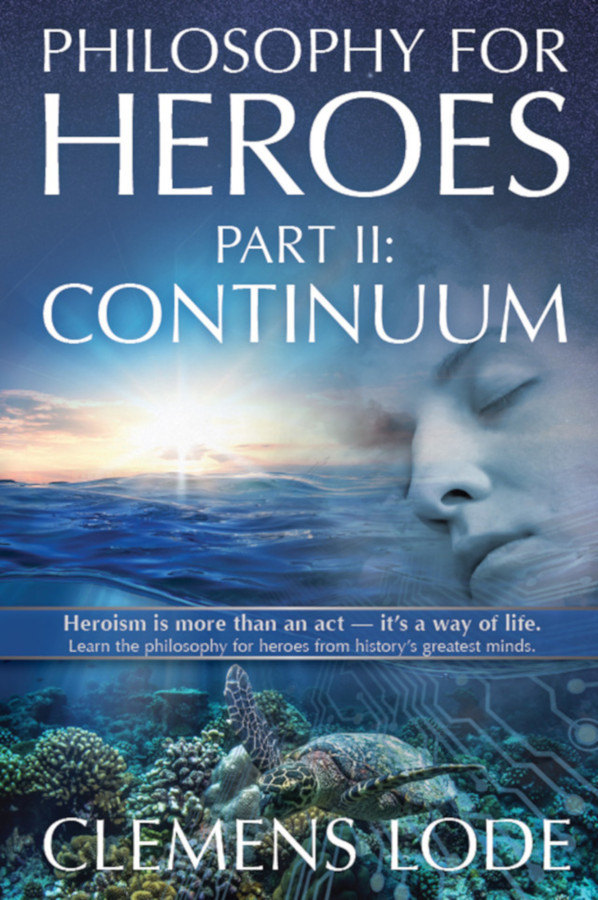
\includegraphics{images/pfh2-cover-900.jpg}
\label{c1_pfh:fig}
\end{figure}

\begin{figure}[H]\centering

\includegraphics{images/Agile_5-11-17_HiRes2-900.jpg}~
\includegraphics{images/KanbanFront_6-28-17_HiRes-900.jpg}
\label{c1_projectmanagement:fig}
\end{figure}

% Remove the following section if you only want to show your covers, replace with your own book descriptions. The example entries are books I have written using this template.


Here are other books by YOUR NAME. All share the topics of philosophy, psychology, leadership, and project management.

\begin{setlength}{\leftmargin}{1cm} 
\begin{description}\setlength{\itemsep}{-5pt}

\item[Better Books with LaTeX] In \citetitle{BBWL}\index{@\citetitle{BBWL}}\ifxetex\else{} \citep{BBWL}\fi, author Clemens Lode provides you a short-cut into the world of book publishing with \LaTeX{}. It is not a book that just lists all the commands and then leave you alone, it guides you alongside a fully working template (this one!).

\item[Part I: Knowledge.] In \citetitle{PFH1E}\index{@\citetitle{PFH1E}}\ifxetex\else{} \citep{PFH1E}\fi, the first book in this four-book series, author Clemens Lode takes the reader on a journey, examining the foundations of knowledge. What is the basis of our understanding of the world? How does society define a ``hero''? How do basic skills, such as language and mathematics, train our way of thinking and reasoning?

\item[Part II: Continuum.] Beyond the static world of the first book, \citetitle{PFH2E}\index{@\citetitle{PFH2E}}\ifxetex\else{} \citep{PFH2E}\fi{} looks at gradual transitions from one condition to the next. Where do we come from? Why is there something rather than nothing? What is the source of our creativity? How can the study of natural sciences help us to understand who we are?

\item[Scrum Your Jira!] In \citetitle{scrum-your-jira}\index{@\citetitle{scrum-your-jira}}\ifxetex\else{} \citep{scrum-your-jira}\fi, author Clemens Lode challenges two illusions that can get in the way of your company's road to being truly Agile: first, that your Scrum is ``special,'' and second, that you can hide behind project management software. Jira is powerful\emdash{}and this book will show you how to use it more effectively\emdash{}but it makes it easy to forget that the first idea of Agile is: Individuals and interactions over processes and tools.

\item[Kanban Remastered] StarCraft, the most popular real-time strategy game of all time, is also all about producing and deploying just as many game units at just the right time. This book is about the relationship of StarCraft and Kanban. When your team knows StarCraft but not Kanban, \citetitle{kanban-remastered}\index{@\citetitle{kanban-remastered}}\ifxetex\else{} \citep{kanban-remastered}\fi{} will provide you with a series of analogies to allow a better and easier understanding of Agile principles. It is written in a light-hearted tone, similar to how you might chat with a fellow coach about your Agile experiences implementing Kanban, taking for granted that you have experience with StarCraft.

\end{description}
\end{setlength}\blankpage

% list of uncited references that are still good reads (only for printed PDF)
\ifxetex
	%%%%%%%%%%%%%%%%%%%%%%%%%%%%%%%%%%%%%
% Read the /ReadMeFirst/ReadMeFirst.tex for an introduction. Check out the accompanying book "Better Books with LaTeX" for a discussion of the template and step-by-step instructions. The template was originally created by Clemens Lode, LODE Publishing (www.lode.de), mail@lode.de, 8/17/2018. Feel free to use this template for your book project!
%%%%%%%%%%%%%%%%%%%%%%%%%%%%%%%%%%%%%

% list of uncited references that are still good reads (only for printed PDF). Replace the citations accordingly.

\nocite{PFH1E}
\nocite{PFH2E}
\nocite{PFH3E}
\nocite{PFH4E}

\printbibliography[keyword=recommendedEN, title={Recommended Reading}]\blankpage
\fi

%%%%%%%%%%%%%%%%%%%%%%%%%%%%%%%%%%%%%
% Read the /ReadMeFirst/ReadMeFirst.tex for an introduction. Check out the accompanying book "Better Books with LaTeX" for a discussion of the template and step-by-step instructions. The template was originally created by Clemens Lode, LODE Publishing (www.lode.de), mail@lode.de, 8/17/2018. Feel free to use this template for your book project!
%%%%%%%%%%%%%%%%%%%%%%%%%%%%%%%%%%%%%


% Upload hires (author_highres.png) and lowres picture (author.jpg) of author into images folder, and uncomment the 5 includegraphics lines.
% Replace quotation text
% Add text describing your motivation, your professional background, what you are currently doing, and how to connect with you.

\begin{chapterpage}{
	{The Author}
}{p1_the-author:cha}

\vspace*{\fill}

\begin{center}

%\ifxetex
%	\includegraphics[width=.7\textwidth]{images/author_hires.png}
%\else
%	\includegraphics{images/author.jpg}
%\fi

\end{center}
\vspace*{\fill}

\begin{myquotation} Viver, morrer, renascer. Progredir sempre. Amar a Deus sobre todas as coisas e ao próximo como a Si mesmo. Buscai em primeiro lugar o Reino de Deus e tudo o mais vos será acrescentado.\end{myquotation}

\end{chapterpage}

Describe your dreams, what goals you have in life, where you went to school or studied, and what job you currently work or worked in the past. Make clear what motivated you to start writing. Finally, add contact points where people can connect with you (mail, Facebook, Twitter, etc.). 
\blankpage
%%%%%%%%%%%%%%%%%%%%%%%%%%%%%%%%%%%%%
% Read the /ReadMeFirst/ReadMeFirst.tex for an introduction. Check out the accompanying book "Better Books with LaTeX" for a discussion of the template and step-by-step instructions. The template was originally created by Clemens Lode, LODE Publishing (www.lode.de), mail@lode.de, 8/17/2018. Feel free to use this template for your book project!
%%%%%%%%%%%%%%%%%%%%%%%%%%%%%%%%%%%%%

% Use this chapter to summarize what you have learned while writing the book. This helps you to write better books in the future and might be interesting for the reader to know about how the book came about.

\begin{chapterpage}{The Book's Story}{p2_booksstory:cha}

% Add a quotation to set the team for your lessons learned
Este livro nasceu da proposta da minha psicóloga Fernanda Volpe Cunha de eu escrever sobre meus pensamentos e sentimentos para poder levar a ela todo esse conteúdo. Aconteceu que foi mais que isso pois os assuntos pessoais levo a ela contudo os de interesse geral partilho aqui.

Acredito piamente que as pessoas precisam desenvolver senso crítico-filosófico e precisam de auto-conhecimento. O que escrevo aqui, não tenho a pretensão de afirmar que é a verdade absoluta pois verdade absoluta só Deus conhece. Mas cada um refletindo sobre os conteúdos, seja concordando ou discordando, encontrará meios de desenvolver-se como uma musculação para a mente e então ficará mais forte para a Vida, esse o objetivo da presente obra.

\end{chapterpage}



\blankpage


% switch back to basic chapter design
%  Reset the chapter design to a basic one (no box, just underlined chapter title---used for the back and front matter)

\renewcommand*\chapterheadstartvskip{\vspace*{-3\topskip}} 
\renewcommand*\chapterheadendvskip{
  \vskip-.5\baselineskip
  \noindent
  {\color{gray}\rule{\linewidth}{2pt}}
  \par}
\renewcommand*\chapterformat{}
\renewcommand*{\chapterpagestyle}{empty}

% needs to be in curly braces because parskip change.
{
\parskip=5pt
%%%%%%%%%%%%%%%%%%%%%%%%%%%%%%%%%%%%%
% Read the /ReadMeFirst/ReadMeFirst.tex for an introduction. Check out the accompanying book "Better Books with LaTeX" for a discussion of the template and step-by-step instructions. The template was originally created by Clemens Lode, LODE Publishing (www.lode.de), mail@lode.de, 8/17/2018. Feel free to use this template for your book project!
%%%%%%%%%%%%%%%%%%%%%%%%%%%%%%%%%%%%%

\chapter{Reflection}

\begin{problem}
Introductory text about what this section is about. For example, describe that this is a summary of all the problem boxes throughout the book and point to an online forum where readers can discuss them.\end{problem}

% Reset formatting
\setlength{\parindent}{0.0cm}
\renewcommand{\index}[1]{}
\renewenvironment{problem}[1][]{$\bullet$\ #1}
\footnotesize 


\section*{Replace with Your First Chapter}
% Add questions located in your first chapter.
\begin{problem}What is LaTeX?\end{problem}


\section*{Replace with Your Second Chapter}
% Add questions located in your second chapter.
\begin{problem}What is LaTeX?\end{problem}


\section*{Replace with Your Third Chapter}
% Add questions located in your third chapter.
\begin{problem}What is LaTeX?\end{problem}
\newpage
%%%%%%%%%%%%%%%%%%%%%%%%%%%%%%%%%%%%%
% Read the /ReadMeFirst/ReadMeFirst.tex for an introduction. Check out the accompanying book "Better Books with LaTeX" for a discussion of the template and step-by-step instructions. The template was originally created by Clemens Lode, LODE Publishing (www.lode.de), mail@lode.de, 8/17/2018. Feel free to use this template for your book project!
%%%%%%%%%%%%%%%%%%%%%%%%%%%%%%%%%%%%%

\chapter{Eureka!}

\begin{idea}
Introductory text about what this section is about. For example, describe that this is a summary of all the idea boxes throughout the book.\end{idea}

% reformat idea boxes
\renewenvironment{idea}[1][]{$\bullet$\ #1}
%\setlength{\parindent}{0.7cm}

% deactivate indexing of idea boxes to prevent duplicates
\ifxetex
	\renewcommand{\index}{}
\fi

\section*{Replace with Your First Chapter}
% Add ideas located in your first chapter.
\begin{idea}
\LaTeX{} is a document preparation system.
\end{idea}

\section*{Replace with Your Second Chapter}
% Add ideas located in your second chapter.
\begin{idea}
\LaTeX{} is a document preparation system.
\end{idea}

\section*{Replace with Your Third Chapter}
% Add ideas located in your third chapter.
\begin{idea}
\LaTeX{} is a document preparation system.
\end{idea}\newpage
\parskip=0pt
%%%%%%%%%%%%%%%%%%%%%%%%%%%%%%%%%%%%%
% Read the /ReadMeFirst/ReadMeFirst.tex for an introduction. Check out the accompanying book "Better Books with LaTeX" for a discussion of the template and step-by-step instructions. The template was originally created by Clemens Lode, LODE Publishing (www.lode.de), mail@lode.de, 8/17/2018. Feel free to use this template for your book project!
%%%%%%%%%%%%%%%%%%%%%%%%%%%%%%%%%%%%%


% If you have added or removed any entries in the glossary directory, add them here. If a letter is missing, add a new \section*{} with the letter.

\chapter{Glossary}

% Special formatting for glossary 
\setlength{\parindent}{0.7cm}
\renewcommand{\index}[1]{}
\renewenvironment{definition}[2][]{\textbf{#2}\ $\bullet$\ #1}
\footnotesize
%\ifxetex
%	\titlespacing*{\section}{0pt}{3.5ex plus 1ex minus .2ex}{2.3ex plus .2ex}
%\fi

\vspace{20pt}


\section*{E}
\begin{multicols}{2}
\begin{definition}{Entity}\index{entity|textbf} An \emph{entity} is a ``thing'' with properties (an identity). For example, a plant produces oxygen, a stone has a hard surface, etc.).\end{definition}
\end{multicols}

\section*{I}
\begin{multicols}{2}
\begin{definition}{Identity}\index{identity|textbf} An \emph{identity} is the sum total of all properties\index{entity!property} of an entity (e.g., weight: 160 pounds, length: 6 feet, has a consciousness, etc.).\end{definition}

\end{multicols}

\section*{L}
\begin{multicols}{2}
\begin{definition}{LaTeX}\index{latex|textbf} \LaTeX{} is a document preparation system.\end{definition}
\end{multicols}

\section*{P}
\begin{multicols}{2}
\begin{definition}{Property}\index{entity!property|textbf} A \emph{property} refers to the manner in which an entity (or a process) affects other entities (or other processes) in a certain situation (e.g., mass, position, length, name, velocity, etc.).\end{definition}
\end{multicols}\newpage
% add separate quotations page (sources in the e-book are already included in the text body)
\ifxetex
	%%%%%%%%%%%%%%%%%%%%%%%%%%%%%%%%%%%%%
% Read the /ReadMeFirst/ReadMeFirst.tex for an introduction. Check out the accompanying book "Better Books with LaTeX" for a discussion of the template and step-by-step instructions. The template was originally created by Clemens Lode, LODE Publishing (www.lode.de), mail@lode.de, 8/17/2018. Feel free to use this template for your book project!
%%%%%%%%%%%%%%%%%%%%%%%%%%%%%%%%%%%%%

% quotation sources (only for print PDF where the source is not directly mentioned in the text body).

\chapter{Quotation Sources}

\setlength{\parindent}{0pt}
\footnotesize

\babelDE{\textbf{\pageref{gogh-sky-quote}:} \cite[vgl.][S.~23--24]{ifyouwanttowrite}}
\babelEN{\textbf{\pageref{gogh-sky-quote}:} \cite[pp.~23--24]{ifyouwanttowrite}}\par
\fi
}

%%%%%%%%%%%%%%%%%%%%%%%%%%%%%%%%%%%%%
% Read the /ReadMeFirst/ReadMeFirst.tex for an introduction. Check out the accompanying book "Better Books with LaTeX" for a discussion of the template and step-by-step instructions. The template was originally created by Clemens Lode, LODE Publishing (www.lode.de), mail@lode.de, 8/17/2018. Feel free to use this template for your book project!
%%%%%%%%%%%%%%%%%%%%%%%%%%%%%%%%%%%%%


% Command to add some text into the bibliography (between the title and the list of referenced books)
% See https://tex.stackexchange.com/questions/197061/text-between-index-or-bibliography-title-and-content
\newcommand{\bibpreface}[1]{\patchcmd{\thebibliography}{\list}{#1\list}{}{}}

\bibpreface{Write here the preface of your list of recommended reading titles. Delete this line to have no preface for this section.}

\ifxetex
	\printbibliography
\else
	\newpage
	\bibliographystyle{plainnat}
	\bibliography{bibliography/english}
\fi


% ---------- Appendix
\appendix
    
%%%%%%%%%%%%%%%%%%%%%%%%%%%%%%%%%%%%%
% Read the /ReadMeFirst/ReadMeFirst.tex for an introduction. Check out the accompanying book "Better Books with LaTeX" for a discussion of the template and step-by-step instructions. The template was originally created by Clemens Lode, LODE Publishing (www.lode.de), mail@lode.de, 8/17/2018. Feel free to use this template for your book project!
%%%%%%%%%%%%%%%%%%%%%%%%%%%%%%%%%%%%%

% the index page, only for printed PDF

\ifxetex	
	\pagestyle{empty}
	\appendix
	\indexprologue{Replace index prologue with an own introduction of how to contact you when there is an errata concerning the index.}
    \printindex
\fi

%%%%%%%%%%%%%%%%%%%%%%%%%%%%%%%%%%%%%
% Read the /ReadMeFirst/ReadMeFirst.tex for an introduction. Check out the accompanying book "Better Books with LaTeX" for a discussion of the template and step-by-step instructions. The template was originally created by Clemens Lode, LODE Publishing (www.lode.de), mail@lode.de, 8/17/2018. Feel free to use this template for your book project!
%%%%%%%%%%%%%%%%%%%%%%%%%%%%%%%%%%%%%


% Replace it with your own call to action if you like, or use the default text.

\chapter{An Important Final Note}

% Only show for e-books.
\ifxetex \else \textit{If you want to rate this e-book, please also add a short text comment. Without a text comment, your star rating will be invisible on the Amazon website and count only as an indicator for further recommendations on Amazon. Thanks!}\fi

Writers are not performance artists. While there are book signings and public readings, most writers (and readers) follow their passion alone in their homes.

\textit{What applause is for the musician, \textbf{reviews} are for the writer.} 

\textit{Books create a community among readers}; you can share your thoughts among all those who will or have read the book.

\textbf{Leave a thoughtful honest review and help me to create such a community on the platform on which you have acquired this book.} \textit{What did you like, what can be improved? To whom would you recommend it?} 

Thank you, also in the name of all the other readers who will be able to better decide whether this book is right for them or not! A positive review will increase the reach of the book, a negative review will improve the quality of the next book. I welcome both!
%%%%%%%%%%%%%%%%%%%%%%%%%%%%%%%%%%%%%
% Read the /ReadMeFirst/ReadMeFirst.tex for an introduction. Check out the accompanying book "Better Books with LaTeX" for a discussion of the template and step-by-step instructions. The template was originally created by Clemens Lode, LODE Publishing (www.lode.de), mail@lode.de, 8/17/2018. Feel free to use this template for your book project!
%%%%%%%%%%%%%%%%%%%%%%%%%%%%%%%%%%%%%

% Replace quote

\newpage
\thispagestyle{empty}
\vspace*{\fill}
\hfill

\babelEN{\begin{myquotation} Deus abençoe a todos\par\mbox{}\hfill \emdash{}Geraldo Cesar Cantelli\end{myquotation}}

\end{document}